\documentclass[12pt]{article}


\usepackage{amssymb}
\usepackage{amsmath}
\usepackage{fullpage}
\usepackage{epsfig}
\usepackage{epstopdf, xcolor, hyperref}
\everymath{\displaystyle}



\begin{document}

\begin{center}
\underline{\LARGE{Integration by Parts}}
\end{center}

\noindent SUGGESTED REFERENCE MATERIAL:

\bigskip

\noindent As you work through the problems listed below, you should reference Chapter 7.2 of the recommended textbook (or the equivalent chapter in your alternative textbook/online resource) and your lecture notes.

\bigskip

\noindent EXPECTED SKILLS:

\begin{itemize}

\item Be able to use integration by parts to evaluate various integrals, including integrands involving products of functions, isolated logarithmic functions, or isolated inverse trigonometric functions.

\end{itemize}

\noindent PRACTICE PROBLEMS:

\medskip

\noindent {\bf For problems 1-12, evaluate the given integral.}

\begin{enumerate}

\item $\int xe^{4x}\,dx$ 

\includegraphics[scale=0.5]{start.pdf}
{{$\frac{x}{4}e^{4x}-\frac{1}{16}e^{4x}+C$}}
\includegraphics[scale=0.5]{end.pdf}


\item $\int x^2\cos{(x)}\,dx$ 

\includegraphics[scale=0.5]{start.pdf}
{{$x^2\sin{x}+2x\cos{x}-2\sin{x}+C$}}
\includegraphics[scale=0.5]{end.pdf}


\item $\int x^2\ln{(x)}\,dx$ 

\includegraphics[scale=0.5]{start.pdf}
{{$\frac{1}{3}x^3\ln{x}-\frac{1}{9}x^3+C$}}
\includegraphics[scale=0.5]{end.pdf}


\item $\int{\frac{\ln{x}}{x^4}} \,dx$

\includegraphics[scale=0.5]{start.pdf}
{{$-\frac{1}{3}x^{-3}\ln{x}-\frac{1}{9}x^{-3}+C$}}
\includegraphics[scale=0.5]{end.pdf}


\item $\int \arcsin{(x)}\,dx$ 

\includegraphics[scale=0.5]{start.pdf}
{{$x\arcsin{x}+\sqrt{1-x^2}+C$}}
\includegraphics[scale=0.5]{end.pdf}


\item $\int x\sec^2{(x)}\,dx$ 

\includegraphics[scale=0.5]{start.pdf}
{{$x\tan{x}+\ln{|\cos{x}|}+C$}}
\includegraphics[scale=0.5]{end.pdf}


\item $\int \ln{(x^2+10)}\,dx$ 

\includegraphics[scale=0.5]{start.pdf}
{{$x\ln{(x^2+10)}-2x+2\sqrt{10}\arctan{\left(\frac{x}{\sqrt{10}}\right)}+C$; Detailed Solution: \textcolor{blue}{\href{http://www.math.drexel.edu/classes/Calculus/resources/Math122HW/Solutions/122_11_Parts_07.pdf}{Here}}}}
\includegraphics[scale=0.5]{end.pdf}


\item $\int e^{2x}\cos{(3x)}\,dx$ 

\includegraphics[scale=0.5]{start.pdf}
{{$\frac{2}{13}e^{2x}\cos{(3x)}+\frac{3}{13}e^{2x}\sin{(3x)}+C$; Detailed Solution: \textcolor{blue}{\href{http://www.math.drexel.edu/classes/Calculus/resources/Math122HW/Solutions/122_11_Parts_08.pdf}{Here}}}}
\includegraphics[scale=0.5]{end.pdf}


\item $\int x\arctan{(x)}\,dx$

\includegraphics[scale=0.5]{start.pdf}
{{$\frac{x^2}{2}\tan^{-1}x-\frac{x}{2}+\frac{1}{2}\tan^{-1}x+C$}}
\includegraphics[scale=0.5]{end.pdf}


\item $\int x^3 \cos{(x^2)} \,dx$

\includegraphics[scale=0.5]{start.pdf}
{{$\frac{1}{2}\cos{(x^2)}+\frac{1}{2}x^2\sin{(x^2)}+C$}}
\includegraphics[scale=0.5]{end.pdf}


\item $\int_{0}^{\pi}3x\sin{(x)}\,dx$ 

\includegraphics[scale=0.5]{start.pdf}
{{$3\pi$; Detailed Solution: \textcolor{blue}{\href{http://www.math.drexel.edu/classes/Calculus/resources/Math122HW/Solutions/122_11_Parts_11.pdf}{Here}}}}
\includegraphics[scale=0.5]{end.pdf}


\item $\int_{0}^{1}x^2e^{x}\,dx$ 

\includegraphics[scale=0.5]{start.pdf}
{{$e-2$}}
\includegraphics[scale=0.5]{end.pdf}


\item Suppose that $u$ and $v$ are differentiable functions of $x$ with $\int_{x=0}^{x=1} v \,du = 3$ and the following functional values.\\
\begin{center}
\begin{tabular}{|c|c|c|}
\hline
$x$ & $u(x)$ & $v(x)$\\
\hline
0 & 5 & 2 \\
\hline
1 & 7 & $-4$\\
\hline
\end{tabular}
\end{center}
Use this information to compute $\int_{x=0}^{x=1} u \,dv$.

\includegraphics[scale=0.5]{start.pdf}
{{$-41$}}
\includegraphics[scale=0.5]{end.pdf}


\item Evaluate $\int \sin{\sqrt{x}} \,dx$ by first making an appropriate substitution and then applying integration by parts.

\includegraphics[scale=0.5]{start.pdf}
{{$2\sin{(\sqrt{x})}-2\sqrt{x}\cos{(\sqrt{x})}+C$}}
\includegraphics[scale=0.5]{end.pdf}


\item Evaluate $\int \left(\sin^{-1}x\right)^2 \,dx$

\includegraphics[scale=0.5]{start.pdf}
{{$x\left(\sin^{-1}x\right)^2-2x+2\sqrt{1-x^2}\left(\sin^{-1}x\right)+C$}}
\includegraphics[scale=0.5]{end.pdf}


\item Find the area of the region which is enclosed by $y=\ln{x}$, $y=1$, and $x=e^2$.

\includegraphics[scale=0.5]{start.pdf}
{{$e$}}
\includegraphics[scale=0.5]{end.pdf}


\item Let $R$ be the region enclosed by the graphs of $y=\ln{x}$, $x=e$, and the $x$-axis (as shown below).

\begin{center}
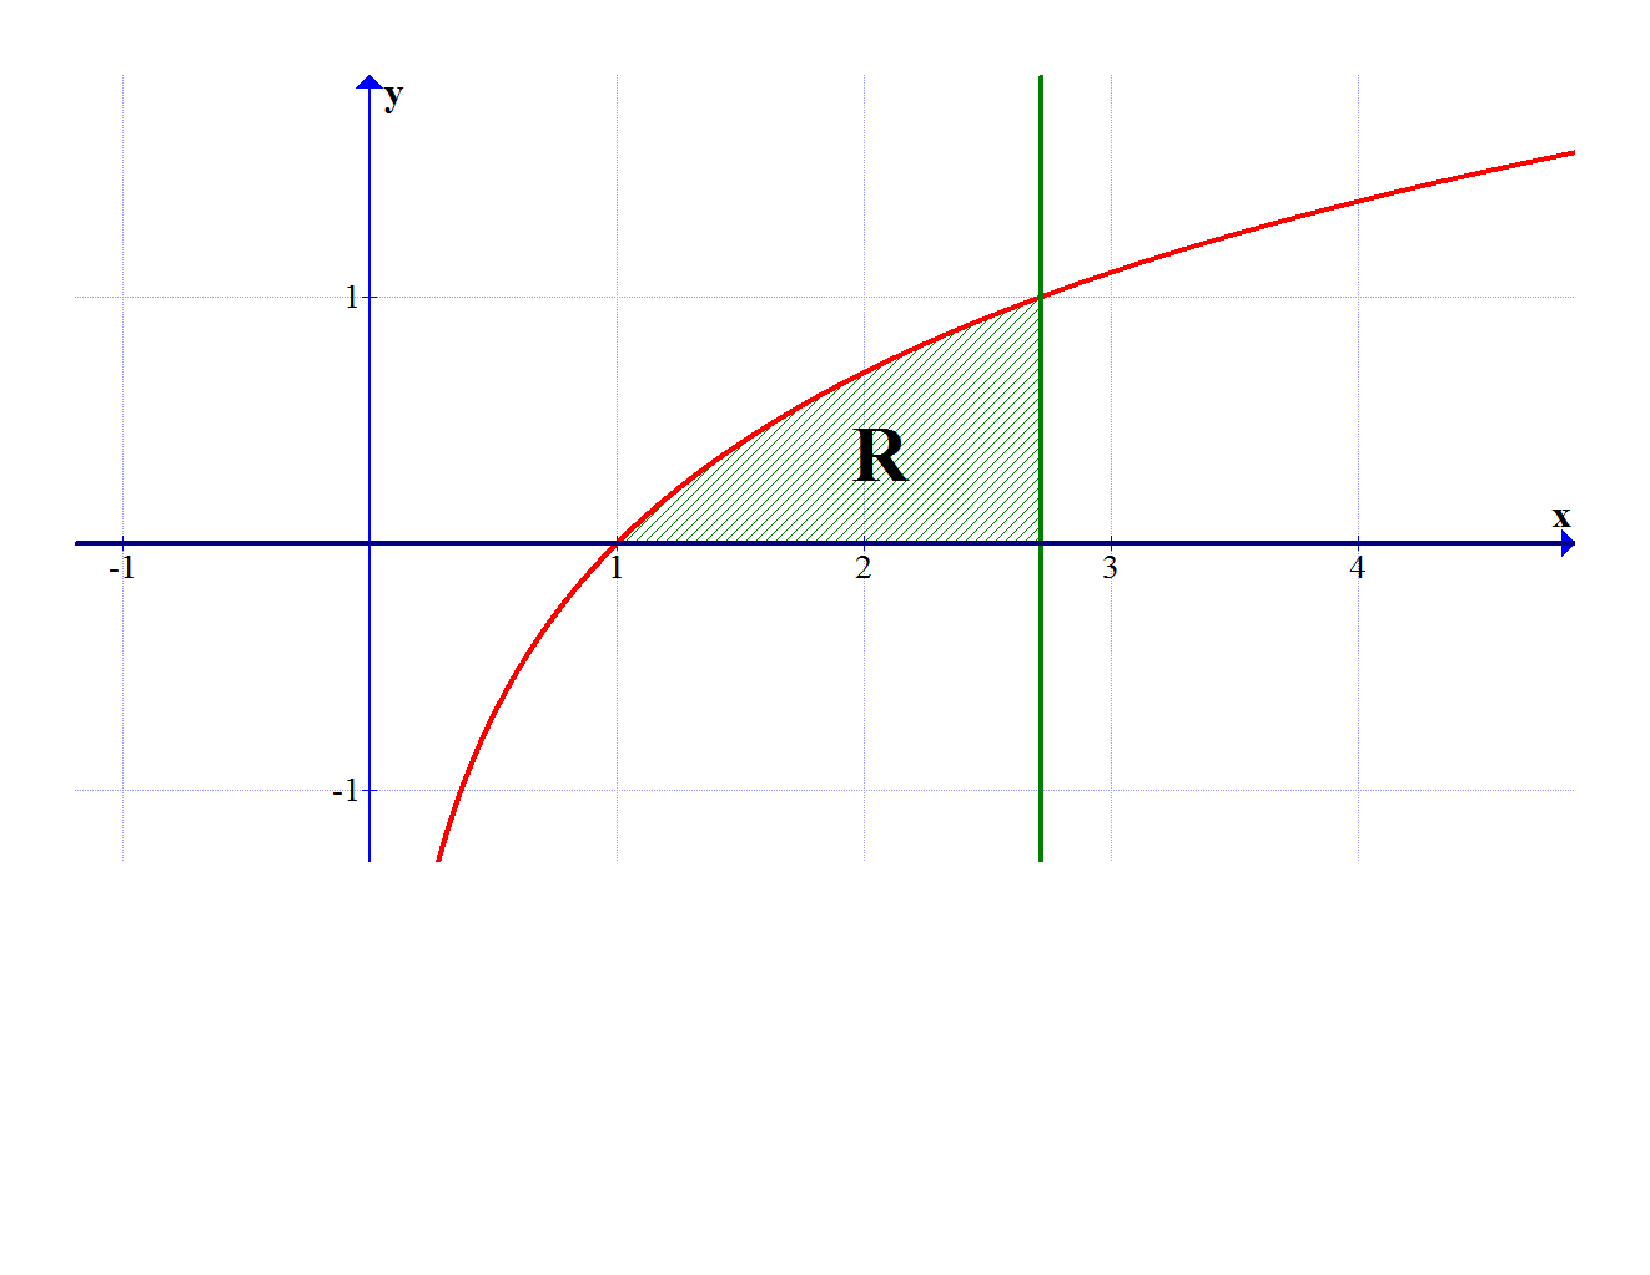
\includegraphics[scale=0.4]{volume2.pdf}
\end{center}

 Find the volume of the solid that results from revolving $R$ around the line $y=-1$.

\includegraphics[scale=0.5]{start.pdf}
{{$\pi e$}}
\includegraphics[scale=0.5]{end.pdf}


\item Let $f$ be a differentiable function. Use integration by parts to show: 
$$\int f(x) \,dx=xf(x)-\int x f^{\prime}(x) \,dx$$

\includegraphics[scale=0.5]{start.pdf}
{{{1\linewidth}{Consider $\int f(x) \,dx$.  Let $u=f(x)$ and $dv=dx$.  Then, $du=f^{\prime}(x)dx$ and $v=x$.  And, integration by parts yields $\int f(x) \,dx = xf(x)-\int x f^{\prime}(x) \,dx$, as desired.}}}
\includegraphics[scale=0.5]{end.pdf}


\end{enumerate}

\end{document}